% ----------------------------------------------------------------------
%
%        Vorlage für Abschlussarbeiten am Lehrstuhl Informatik XII
%
%                   http://ls12-www.cs.uni-dortmund.de
%
%   Für Fragen und Anregungen zur Vorlage: info@ls12.cs.uni-dortmund.de
%
%   Stand: 03.09.2013
%
% ----------------------------------------------------------------------

\RequirePackage{ifthen}

\newcommand \type{Fachprojekt Report}
\newcommand \Autor{Firstname~Lastname}
\newcommand \submissiondate{Sbumission Date}
\newcommand \thesistitle{Title of the Report}
\newcommand \firstsupervisor{Prof.~Dr. Jian-Jia Chen}
\newcommand \secondsupervisor{M.Sc. Junjie Shi}
\newcommand \ErstLehrstuhl{Lehrstuhl Informatik 12 (Eingebettete Systeme) \\ \url{http://ls12-www.cs.tu-dortmund.de}}
\newcommand \ZweitLehrstuhl{}

\RequirePackage{ifpdf} \ifpdf
  \pdfoutput=1
  \pdftrue
  \message{pdfLaTeX}
  \documentclass[pdftex,11pt,a4paper,twoside,ngerman]{scrbook}
  \usepackage{float}
  \usepackage[pdftex]{thumbpdf}
  \usepackage[pdftex]{graphicx}
  \usepackage[pdftex]{hyperref}
  \usepackage{pdfpages}
  \pdfoutput=1
  \pdfcompresslevel=9
  \DeclareGraphicsExtensions{.pdf,.jpg,.png}
\else
  \pdffalse
  \message{LaTeX}
  \documentclass[dvips,11pt,a4paper,twoside,ngerman]{scrbook}
  \usepackage{float}
  \usepackage{graphicx}
  \usepackage{epsf}
  \usepackage[dvips]{hyperref}
  \DeclareGraphicsExtensions{.eps}
\fi

% Informationen fuer pdf-File festlegen
\hypersetup
{
    pdfauthor = {\Autor},
    pdftitle = {\thesistitle},
    pdfsubject = {\type, TU Dortmund, Fakult{\"a}t f{\"u}r Informatik},
    pdfproducer = {LaTeX},
    pdfview = FitV,
    pdfstartview = FitV,
    pdfhighlight = /I,
    pdfborder = 0 0 0,
    colorlinks = false,
    bookmarksopen,
    bookmarksopenlevel = 1,
    bookmarksnumbered = false,
    plainpages = false
}%

% -------------------------------------------------------------------
% Seitenformat anpassen
\usepackage[a4paper,left=3.5cm,right=2.5cm,bottom=3.5cm,top=3cm]{geometry}
\setlength{\headheight}{15pt}

% -------------------------------------------------------------------
% Grafikpakete einbinden
\usepackage{amsmath,amssymb}
\usepackage{flafter}
\usepackage{subfigure}

% -------------------------------------------------------------------
\usepackage{ifthen}

% -------------------------------------------------------------------
\usepackage[absolute,overlay]{textpos}
\setlength{\TPHorizModule}{1mm}
\setlength{\TPVertModule}{\TPHorizModule}
\textblockorigin{0mm}{0mm}
\usepackage{fix-cm}
\usepackage{setspace}
\usepackage{scrhack}

% -------------------------------------------------------------------
% Korrekte Darstellung der Umlaute
% \usepackage[german,ngerman]{babel}
% \usepackage[utf8]{inputenc}
% \usepackage[T1]{fontenc}
% \usepackage{ae,aecompl}

% -------------------------------------------------------------------
% Bibtex deutsch
%\usepackage[numbers,sort,square]{natbib}
%\usepackage{bibgerm}

% -------------------------------------------------------------------
% Anführungszeichen
\usepackage[babel,german=quotes]{csquotes}

% -------------------------------------------------------------------
% URLs
\usepackage{url}

% -------------------------------------------------------------------
% Caption anpassen
\usepackage[margin=0pt,font=small,labelfont=bf]{caption}

% -------------------------------------------------------------------
% Erweitere Tabellen
\usepackage{booktabs}

% -------------------------------------------------------------------
% Eurosymbol
\usepackage{eurosym}

% -------------------------------------------------------------------
% Zeilenabstand einstellen
\renewcommand{\baselinestretch}{1.25}
% Floating-Umgebungen anpassen
\renewcommand{\topfraction}{0.9}
\renewcommand{\bottomfraction}{0.8}

% -------------------------------------------------------------------
% Keine einzelnen Zeilen beim Anfang eines Abschnitts ("Schusterjungen")
\clubpenalty = 10000
% Keine einzelnen Zeilen am Ende eines Abschnitts ("Hurenkinder")
\widowpenalty = 10000 \displaywidowpenalty = 10000
\parindent=0cm

% -------------------------------------------------------------------
% Kopfzeile hinzufuegen
\usepackage{fancyhdr}
\usepackage{extramarks}

\pagestyle{fancy}
\renewcommand{\chaptermark}[1]{\markboth{#1}{}}
\renewcommand{\sectionmark}[1]{\markright{#1}{}}

\fancyhf{}
\fancyhead[LE,RO]{\thepage}
\fancyhead[RE]{\textit{\nouppercase{\leftmark}}}
\fancyhead[LO]{\textit{\nouppercase{\rightmark}}}

\fancypagestyle{plain}{ %
\fancyhf{} % remove everything
\renewcommand{\headrulewidth}{0pt} % remove lines as well
\renewcommand{\footrulewidth}{0pt}} \pagestyle{headings}

% -------------------------------------------------------------------
% Eigene Farben definieren
\usepackage{color}
\definecolor{TUGreen}{rgb}{0.517,0.721,0.094}
\definecolor{TUOrange}{rgb}{1.0,0.7176,0.0}
\definecolor{BrightGray}{gray}{0.9}
\definecolor{DarkGray}{gray}{0.2}
\definecolor{white}{rgb}{1,1,1}
\definecolor{black}{rgb}{0,0,0}
\definecolor{red}{rgb}{1,0,0}

% -------------------------------------------------------------------
% Programm-Listings einbinden und formatieren
\usepackage{listings}

\lstdefinestyle{C++}
{
language=C++,
backgroundcolor=\color{BrightGray},
keywordstyle=\tt\bfseries,  %\color{TUGreen}\bfseries,
commentstyle=\color{DarkGray},
stringstyle=\color{red},
showstringspaces=false,
basicstyle=\small\color{black},
numbers=left,
captionpos=b,
tabsize=4,
breaklines=true
}

% -------------------------------------------------------------------
% Algorithmen
\usepackage[plain,chapter]{algorithm}
\usepackage{algorithmic}

\usepackage{enumerate}

% -------------------------------------------------------------------
% Algorithmen anpassen
\renewcommand{\algorithmicrequire}{\textit{Eingabe:}}
\renewcommand{\algorithmicensure}{\textit{Ausgabe:}}
\floatname{algorithm}{Algorithmus}
\renewcommand{\listalgorithmname}{Algorithmenverzeichnis}
\renewcommand{\algorithmiccomment}[1]{\color{grau}{// #1}}

% -------------------------------------------------------------------
% Theorem-Umgebungen
\usepackage[amsmath,thmmarks]{ntheorem}
\theoremseparator{.}
\theoremstyle{change}
\newtheorem{theorem}{Theorem}[section]
\newtheorem{satz}[theorem]{Satz}
\newtheorem{lemma}[theorem]{Lemma}
\newtheorem{korollar}[theorem]{Korollar}
\newtheorem{proposition}[theorem]{Proposition}
% Ohne Numerierung
\theoremstyle{nonumberplain}
\renewtheorem{theorem*}{Theorem}
\renewtheorem{satz*}{Satz}
\renewtheorem{lemma*}{Lemma}
\renewtheorem{korollar*}{Korollar}
\renewtheorem{proposition*}{Proposition}
% Definitionen mit \upshape
\theorembodyfont{\upshape}
\theoremstyle{change}
\newtheorem{definition}[theorem]{Definition}
\theoremstyle{nonumberplain}
\renewtheorem{definition*}{Definition}
% Kursive Schrift
\theoremheaderfont{\itshape}
\newtheorem{notation}{Notation}
\newtheorem{konvention}{Konvention}
\newtheorem{bezeichnung}{Bezeichnung}
\theoremsymbol{\ensuremath{\Box}}
\newtheorem{beweis}{Beweis}
\theoremsymbol{}
\theoremstyle{change}
\theoremheaderfont{\bfseries}
\newtheorem{bemerkung}[theorem]{Bemerkung}
\newtheorem{beobachtung}[theorem]{Beobachtung}
\newtheorem{beispiel}[theorem]{Beispiel}
\newtheorem{problem}{Problem}
\theoremstyle{nonumberplain}
\renewtheorem{bemerkung*}{Bemerkung}
\renewtheorem{beispiel*}{Beispiel}
\renewtheorem{problem*}{Problem}

% Algorithmen anpassen %
\renewcommand{\algorithmicrequire}{\textit{Eingabe:}}
\renewcommand{\algorithmicensure}{\textit{Ausgabe:}}
\floatname{algorithm}{Algorithmus}
\renewcommand{\listalgorithmname}{Algorithmenverzeichnis}
\renewcommand{\algorithmiccomment}[1]{\color{grau}{// #1}}

% Zeilenabstand einstellen %
\renewcommand{\baselinestretch}{1.25}
% Floating-Umgebungen anpassen %
\renewcommand{\topfraction}{0.9}
\renewcommand{\bottomfraction}{0.8}
% Abkuerzungen richtig formatieren %
\usepackage{xspace}
\newcommand{\vgl}{vgl.\@\xspace} 
\newcommand{\zB}{z.\nolinebreak[4]\hspace{0.125em}\nolinebreak[4]B.\@\xspace}
\newcommand{\bzw}{bzw.\@\xspace}
\newcommand{\dahe}{d.\nolinebreak[4]\hspace{0.125em}h.\nolinebreak[4]\@\xspace}
\newcommand{\etc}{etc.\@\xspace}
\newcommand{\evtl}{evtl.\@\xspace}
\newcommand{\ggf}{ggf.\@\xspace}
\newcommand{\bzgl}{bzgl.\@\xspace}
\newcommand{\so}{s.\nolinebreak[4]\hspace{0.125em}\nolinebreak[4]o.\@\xspace}
\newcommand{\iA}{i.\nolinebreak[4]\hspace{0.125em}\nolinebreak[4]A.\@\xspace}
\newcommand{\sa}{s.\nolinebreak[4]\hspace{0.125em}\nolinebreak[4]a.\@\xspace}
\newcommand{\su}{s.\nolinebreak[4]\hspace{0.125em}\nolinebreak[4]u.\@\xspace}
\newcommand{\ua}{u.\nolinebreak[4]\hspace{0.125em}\nolinebreak[4]a.\@\xspace}
\newcommand{\og}{o.\nolinebreak[4]\hspace{0.125em}\nolinebreak[4]g.\@\xspace}
\newcommand{\oBdA}{o.\nolinebreak[4]\hspace{0.125em}\nolinebreak[4]B.\nolinebreak[4]\hspace{0.125em}d.\nolinebreak[4]\hspace{0.125em}A.\@\xspace}
\newcommand{\OBdA}{O.\nolinebreak[4]\hspace{0.125em}\nolinebreak[4]B.\nolinebreak[4]\hspace{0.125em}d.\nolinebreak[4]\hspace{0.125em}A.\@\xspace}

% Leere Seite ohne Seitennummer, naechste Seite rechts
\newcommand{\blankpage}{
 \clearpage{\pagestyle{empty}\cleardoublepage}
}





\begin{document}

% Titelseite ---------------------------------------------------------
%
\pdfbookmark{Titelpage}{pdf:title}
\pagenumbering{alph}
\pagestyle{empty}
%\selectlanguage{english}
\begin{titlepage}
\definecolor{TUGreen}{rgb}{0.517,0.721,0.094}
\vspace*{-2cm}
\newlength{\links}
\setlength{\links}{-1.5cm}
\sffamily
\hspace*{\links}
\begin{minipage}{12.5cm}

\includegraphics[width=8cm]{bilder/tud_logo_rgb}
%\hspace*{-0.25cm} \textbf{TECHNISCHE UNIVERSIT"AT DORTMUND}\\
%\hspace*{-1.2cm} \rule{5mm}{5mm} \hspace*{0.1cm} FACHBEREICH INFORMATIK\\
\end{minipage}

\vspace*{4cm}

\hspace*{\links}
\hspace*{-0.2cm}
\begin{minipage}{9cm}
\large
\begin{center}
{\Large \type} \\
\vspace*{1cm}
\textbf{\thesistitle} \\
\vspace*{1cm}
\Autor \\
% \vspace*{1cm}
\submissiondate
\end{center}
\end{minipage}
\normalsize
\vspace*{5.5cm}

% \hspace*{\links}

\vspace*{2.1cm}

\hspace*{\links}
\begin{minipage}[b]{8cm}
% \normalsize
\raggedright
Supervisors: \\
\firstsupervisor \\
\secondsupervisor \\
\end{minipage}

\vspace*{2.5cm}
\hspace*{\links}
\begin{minipage}[b]{8cm}
% \normalsize
\raggedright
Technische Universit\"at Dortmund \\
Fakult\"at f\"ur Informatik\\
\ErstLehrstuhl
\end{minipage}


\end{titlepage}

\blankpage


% Inhaltsverzeichnis -------------------------------------------------
%
\pdfbookmark{Table of Content}{pdf:toc}
\pagenumbering{roman}
\tableofcontents
\cleardoublepage
\pagenumbering{arabic}

% Mathematische Notation -----------------------------------------------
%
\pagestyle{empty}
\pdfbookmark{Mathmatic Notation}{pdf:Notation}
%========================================================================================
% TU Dortmund, Informatik Lehrstuhl VII
%========================================================================================

\chapter*{Mathmatical Notation} \label{Notation}

\newcommand{\tabdummy}{\midrule[0pt]}

\begin{tabular}{p{0.25\textwidth}p{0.65\textwidth}}
  \textbf{Notation} & \textbf{Bedeutung} \\ \toprule[1pt]
   $\mathbb{N}$ & Menge der natürlichen Zahlen ${1, 2, 3, \ldots}$ \\ \tabdummy
   $\mathbb{R}$ & Menge der reellen Zahlen \\ \tabdummy
   $\mathbb{R}^d$ & $d$-dimensionaler Raum\\ \tabdummy
   $\mathcal{M} = \{m_1,\ldots,m_N\}$ & Menge $\mathcal{M}$ von $N$ Elementen $m_i$ \\ \tabdummy
   $G=(V,E)$ & Graph $G$ mit Knotenmenge $V$ und Kantenmenge $E$ \\ \tabdummy
   $\mathbf{p}$ & Vektor\\ \tabdummy
   $\mathbf{p}_i$ & $i$-tes Element eines Vektors \\ \tabdummy
   $\mathbf{v}^{(j)}_i$ & $i$-tes Element des $j$-ten Vektors \\ \tabdummy
   $\mathbf{A}$ & Matrix
\end{tabular}

\cleardoublepage

\pagenumbering{arabic}
\pagestyle{fancy} 

% Inhalte --------------------------------------------------------------
%
%========================================================================================
% TU Dortmund, Informatik Lehrstuhl VII
%========================================================================================

\chapter{Einleitung}
\label{Einleitung}

\section{Motivation und Hintergrund}
\label{Motivation_und_Hintergrund}
%
Literatur \cite{Abramowski:1991} oder \cite{Abramowski:1991, Muller:2011} sowie Hinweise auf Quellen im Internet \cite{Khronos:2012} und Verweis auf Kapitel \ref{Kapitel 2} ab Seite \pageref{Kapitel 2}.\\

Hinweise auf Diplom- \cite{Nachname-Diplom:2012}, Bachelor- \cite{Nachname-Bachelor:2012} und Masterarbeiten \cite{Nachname-Master:2012} sind auch möglich.




\section{Aufbau der Arbeit}
\label{Aufbau_der_Arbeit}
%
Er hörte \enquote{leise Schritte} hinter sich. Das bedeutete
nichts Gutes. Wer würde ihm schon folgen, spät in der Nacht und
dazu noch in dieser engen Gasse mitten im übel beleumundeten
Hafenviertel\footnote{Wer würde ihm schon folgen.}? Gerade jetzt, wo er das Ding seines Lebens gedreht
hatte und mit der Beute verschwinden wollte! Hatte einer seiner
zahllosen Kollegen dieselbe Idee gehabt, ihn beobachtet und
abgewartet, um ihn nun um die Früchte seiner Arbeit zu
erleichtern? Oder gehörten die Schritte hinter ihm zu einem der
unzähligen Gesetzeshüter dieser Stadt, und die stählerne Acht um
seine Handgelenke würde gleich zuschnappen? Er konnte die
Aufforderung stehen zu bleiben
schon hören.

Gehetzt sah er sich um. Plötzlich erblickte er den schmalen
Durchgang. Blitzartig drehte er sich nach rechts und verschwand
zwischen den beiden Gebäuden. Beinahe wäre er dabei über den
umgestürzten Mülleimer gefallen, der mitten im Weg lag. Er
versuchte, sich in der Dunkelheit seinen Weg zu ertasten und
erstarrte: Anscheinend gab es keinen anderen Ausweg aus diesem
kleinen Hof als den Durchgang, durch den er gekommen war. Die
Schritte wurden lauter und lauter, er sah eine dunkle Gestalt um
die Ecke biegen. Fieberhaft irrten seine Augen durch die
nächtliche Dunkelheit und suchten einen Ausweg. War jetzt wirklich
alles vorbei, waren alle Mühe und alle Vorbereitungen umsonst?

Er presste sich ganz eng an die Wand hinter ihm und hoffte, der
Verfolger würde ihn übersehen, als plötzlich neben ihm mit kaum
wahrnehmbarem Quietschen eine Tür im nächtlichen Wind hin und her
schwang. Könnte dieses der flehentlich herbeigesehnte Ausweg aus
seinem Dilemma sein? Langsam bewegte er sich auf die offene Tür
zu, immer dicht an die Mauer gepresst. Würde diese Tür seine
Rettung werden? Er hörte leise Schritte hinter sich. Das bedeutete
nichts Gutes. Wer würde ihm schon folgen, spät in der Nacht und
dazu noch in dieser engen Gasse mitten im übel beleumundeten
Hafenviertel? Gerade jetzt, wo er das Ding seines Lebens gedreht
hatte und mit der Beute verschwinden wollte! Hatte einer seiner
zahllosen Kollegen dieselbe Idee gehabt, ihn beobachtet und
abgewartet, um ihn nun um die Früchte seiner Arbeit zu
erleichtern? Oder gehörten die Schritte hinter ihm zu einem der
unzähligen Gesetzeshüter dieser Stadt, und die stählerne Acht um
seine Handgelenke würde gleich zuschnappen? Er konnte die
Aufforderung stehen zu bleiben schon hören. Gehetzt sah er sich
um. Plötzlich erblickte er den schmalen Durchgang. Blitzartig
drehte er sich nach rechts und verschwand zwischen den beiden
Gebäuden.

Er hörte \enquote{leise Schritte} hinter sich. Das bedeutete
nichts Gutes. Wer würde ihm schon folgen, spät in der Nacht und
dazu noch in dieser engen Gasse mitten im übel beleumundeten
Hafenviertel? Gerade jetzt, wo er das Ding seines Lebens gedreht
hatte und mit der Beute verschwinden wollte! Hatte einer seiner
zahllosen Kollegen dieselbe Idee gehabt, ihn beobachtet und
abgewartet, um ihn nun um die Früchte seiner Arbeit zu
erleichtern? Oder gehörten die Schritte hinter ihm zu einem der
unzähligen Gesetzeshüter dieser Stadt, und die stählerne Acht um
seine Handgelenke würde gleich zuschnappen? Er konnte die
Aufforderung stehen zu bleiben
schon hören.

Gehetzt sah er sich um. Plötzlich erblickte er den schmalen
Durchgang. Blitzartig drehte er sich nach rechts und verschwand
zwischen den beiden Gebäuden. Beinahe wäre er dabei über den
umgestürzten Mülleimer gefallen, der mitten im Weg lag. Er
versuchte, sich in der Dunkelheit seinen Weg zu ertasten und
erstarrte: Anscheinend gab es keinen anderen Ausweg aus diesem
kleinen Hof als den Durchgang, durch den er gekommen war. Die
Schritte wurden lauter und lauter, er sah eine dunkle Gestalt um
die Ecke biegen. Fieberhaft irrten seine Augen durch die
nächtliche Dunkelheit und suchten einen Ausweg. War jetzt wirklich
alles vorbei, waren alle Mühe und alle Vorbereitungen umsonst?

Er presste sich ganz eng an die Wand hinter ihm und hoffte, der
Verfolger würde ihn übersehen, als plötzlich neben ihm mit kaum
wahrnehmbarem Quietschen eine Tür im nächtlichen Wind hin und her
schwang. Könnte dieses der flehentlich herbeigesehnte Ausweg aus
seinem Dilemma sein? Langsam bewegte er sich auf die offene Tür
zu, immer dicht an die Mauer gepresst. Würde diese Tür seine
Rettung werden? Er hörte leise Schritte hinter sich. Das bedeutete
nichts Gutes. Wer würde ihm schon folgen, spät in der Nacht und
dazu noch in dieser engen Gasse mitten im übel beleumundeten
Hafenviertel? Gerade jetzt, wo er das Ding seines Lebens gedreht
hatte und mit der Beute verschwinden wollte! Hatte einer seiner
zahllosen Kollegen dieselbe Idee gehabt, ihn beobachtet und
abgewartet, um ihn nun um die Früchte seiner Arbeit zu
erleichtern? Oder gehörten die Schritte hinter ihm zu einem der
unzähligen Gesetzeshüter dieser Stadt, und die stählerne Acht um
seine Handgelenke würde gleich zuschnappen? Er konnte die
Aufforderung stehen zu bleiben schon hören. Gehetzt sah er sich
um. Plötzlich erblickte er den schmalen Durchgang. Blitzartig
drehte er sich nach rechts und verschwand zwischen den beiden
Gebäuden.


\cleardoublepage
%========================================================================================
% TU Dortmund, Informatik Lehrstuhl VII
%========================================================================================

\chapter{Das Kapitel 2}
\label{Kapitel 2}
%
Gehetzt sah er sich um. Plötzlich erblickte er den schmalen
Durchgang. Blitzartig drehte er sich nach rechts und verschwand
zwischen den beiden Gebäuden. Beinahe wäre er dabei über den
umgestürzten Mülleimer gefallen, der mitten im Weg lag. Er
versuchte, sich in der Dunkelheit seinen Weg zu ertasten und
erstarrte: Anscheinend gab es keinen anderen Ausweg aus diesem
kleinen Hof als den Durchgang, durch den er gekommen war.


\section{Kapitel 2 - Unterkapitel 1}
\label{Kapitel_2_-_Unterkapitel_1}
%
Er hörte \enquote{leise Schritte} hinter sich. Das bedeutete
nichts Gutes. Wer würde ihm schon folgen, spät in der Nacht und
dazu noch in dieser engen Gasse mitten im übel beleumundeten
Hafenviertel? Gerade jetzt, wo er das Ding seines Lebens gedreht
hatte und mit der Beute verschwinden wollte! Hatte einer seiner
zahllosen Kollegen dieselbe Idee gehabt, ihn beobachtet und
abgewartet, um ihn nun um die Früchte seiner Arbeit zu
erleichtern? Oder gehörten die Schritte hinter ihm zu einem der
unzähligen Gesetzeshüter dieser Stadt, und die stählerne Acht um
seine Handgelenke würde gleich zuschnappen? Er konnte die
Aufforderung stehen zu bleiben schon hören:

\begin{itemize}
  \item Stop
  \item Stop
  \item Stop.
\end{itemize}

Gehetzt sah er sich um. Plötzlich erblickte er den schmalen
Durchgang. Blitzartig drehte er sich nach rechts und verschwand
zwischen den beiden Gebäuden. Beinahe wäre er dabei über den
umgestürzten Mülleimer gefallen, der mitten im Weg lag. Er
versuchte, sich in der Dunkelheit seinen Weg zu ertasten und
erstarrte: Anscheinend gab es keinen anderen Ausweg aus diesem
kleinen Hof als den Durchgang, durch den er gekommen war. Die
Schritte wurden lauter und lauter, er sah eine dunkle Gestalt um
die Ecke biegen. Fieberhaft irrten seine Augen durch die
nächtliche Dunkelheit und suchten einen Ausweg. War jetzt wirklich
alles vorbei, waren alle Mühe und alle Vorbereitungen umsonst \cite{Abramowski:1991}?



    \begin{figure}[t]
    \centering
    \subfigure[]
          {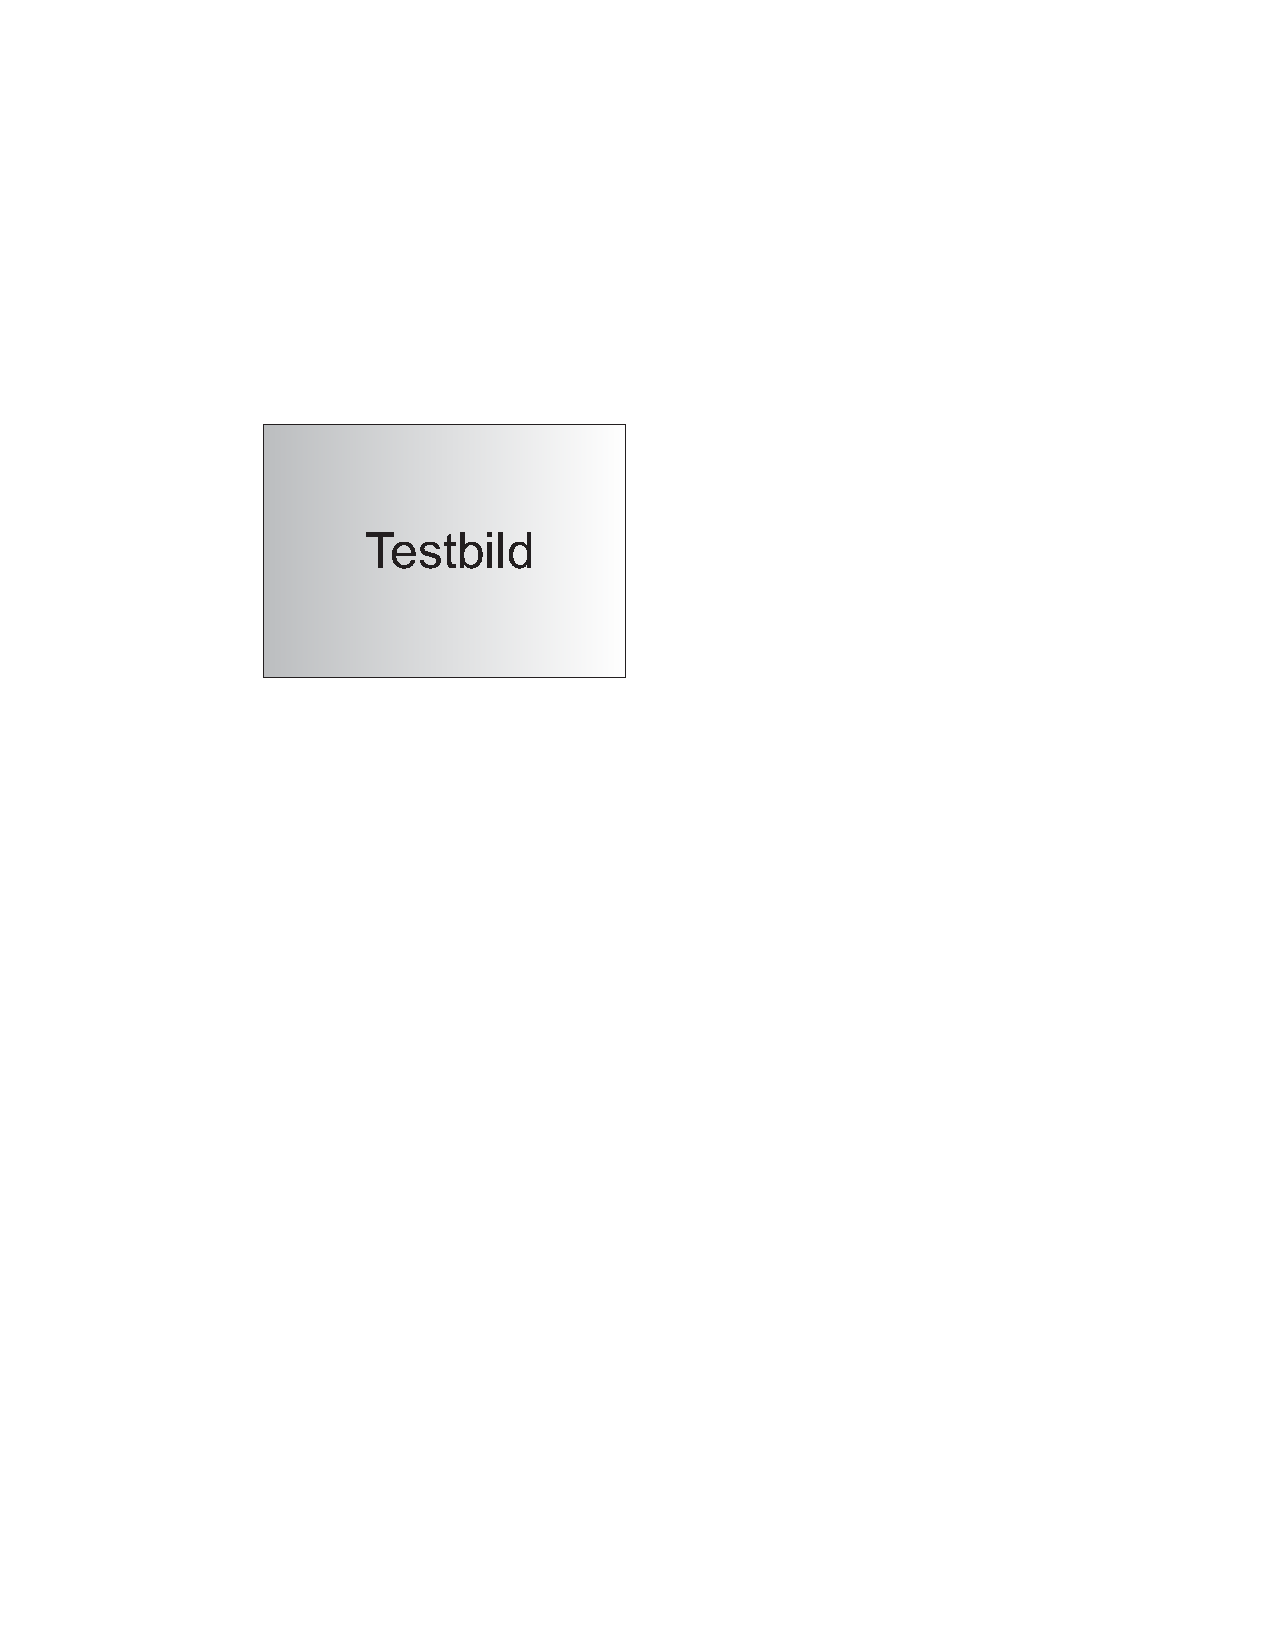
\includegraphics[scale=0.8]{bilder/testbild}\label{fig_testbild_a}
    }
    \hspace{0.5cm}%
    \subfigure[]
         {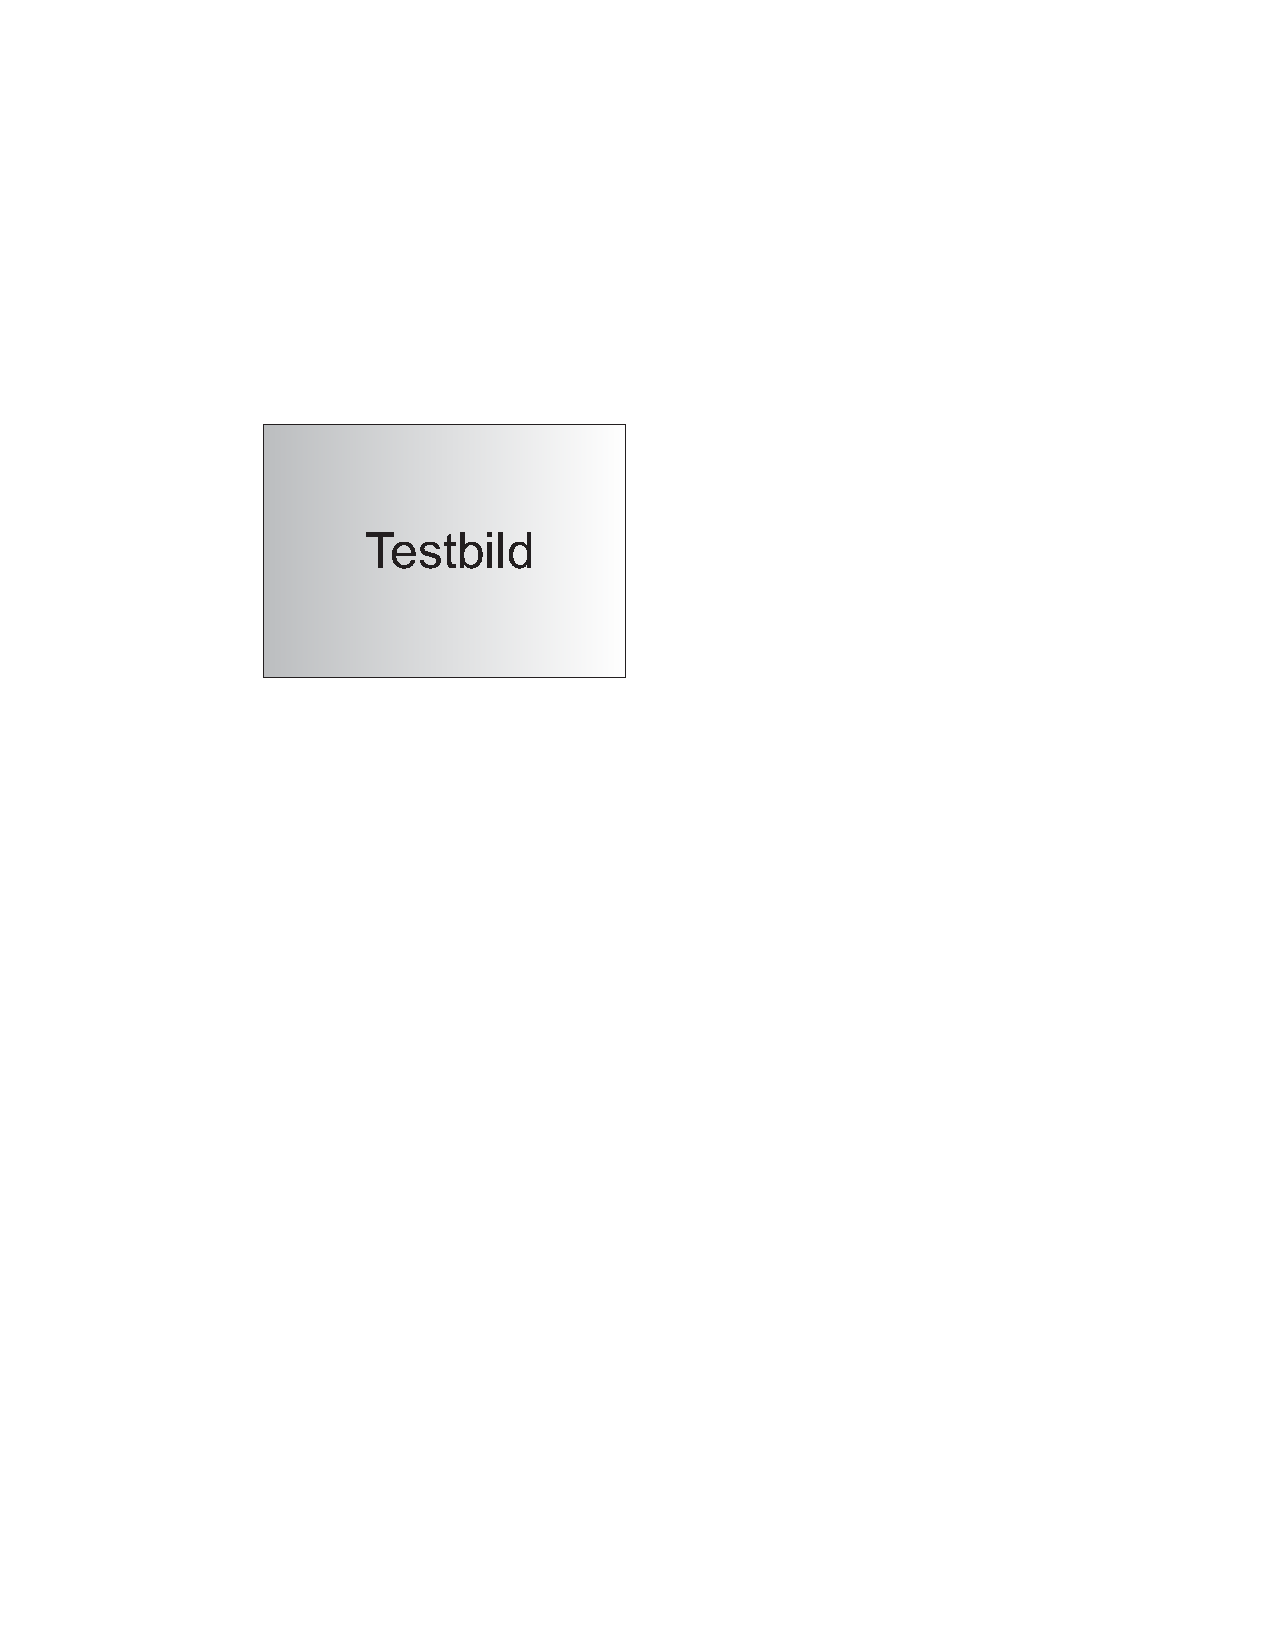
\includegraphics[scale=0.8]{bilder/testbild}\label{fig_testbild_b}
    }
    \caption[Testbilder]{Testbilder}
        \label{fig_testbild}
    \end{figure}

Er presste sich ganz eng an die Wand hinter ihm und hoffte, der
Verfolger würde ihn übersehen, als plötzlich neben ihm mit kaum
wahrnehmbarem Quietschen eine Tür im nächtlichen Wind hin und her
schwang. Könnte dieses der flehentlich herbeigesehnte Ausweg aus
seinem Dilemma sein? Langsam bewegte er sich auf die offene Tür
zu, immer dicht an die Mauer gepresst. Würde diese Tür seine
Rettung werden? Er hörte leise Schritte hinter sich. Das bedeutete
nichts Gutes. Wer würde ihm schon folgen, spät in der Nacht und
dazu noch in dieser engen Gasse mitten im übel beleumundeten
Hafenviertel? Gerade jetzt, wo er das Ding seines Lebens gedreht
hatte und mit der Beute verschwinden wollte! Hatte einer seiner
zahllosen Kollegen dieselbe Idee gehabt, ihn beobachtet und
abgewartet, um ihn nun um die Früchte seiner Arbeit zu
erleichtern? Oder gehörten die Schritte hinter ihm zu einem der
unzähligen Gesetzeshüter dieser Stadt, und die stählerne Acht um
seine Handgelenke würde gleich zuschnappen? Er konnte die
Aufforderung stehen zu bleiben schon hören. Gehetzt sah er sich
um. Plötzlich erblickte er den schmalen Durchgang. Blitzartig
drehte er sich nach rechts und verschwand zwischen den beiden
Gebäuden.


\section{Kapitel 2 - Unterkapitel 2}
\label{Kapitel_2_-_Unterkapitel_2}
%
Er hörte \enquote{leise Schritte} hinter sich. Das bedeutete
nichts Gutes. Wer würde ihm schon folgen, spät in der Nacht und
dazu noch in dieser engen Gasse mitten im übel beleumundeten
Hafenviertel? Gerade jetzt, wo er das Ding seines Lebens gedreht
hatte und mit der Beute verschwinden wollte! Hatte einer seiner
zahllosen Kollegen dieselbe Idee gehabt, ihn beobachtet und
abgewartet, um ihn nun um die Früchte seiner Arbeit zu
erleichtern? Oder gehörten die Schritte hinter ihm zu einem der
unzähligen Gesetzeshüter dieser Stadt, und die stählerne Acht um
seine Handgelenke würde gleich zuschnappen? Er konnte die
Aufforderung stehen zu bleiben schon hören:


    \begin{equation}
        \label{gleichung_nummer_1}
        \mu_{x}(y) = \left\{ \begin{array}{lll}
        4^{\alpha_0} & \qquad \textrm{für} \qquad y \leq 3\\
        \\
        4^{\alpha_1} & \qquad \textrm{für} \qquad y > 3\\
        \end{array} \right.
    \end{equation}
    mit
    \begin{eqnarray}
        \label{gleichung_nummer_2}
        \alpha_0 & = & -\ln 2 \cdot y - \bar{y}\\
        \alpha_1 & = & -\ln 2 \cdot y - \bar{y}\textrm{.}
    \end{eqnarray}



Gehetzt sah er sich um. Plötzlich erblickte er den schmalen
Durchgang. Blitzartig drehte er sich nach rechts und verschwand
zwischen den beiden Gebäuden. Beinahe wäre er dabei über den
umgestürzten Mülleimer gefallen, der mitten im Weg lag. Er
versuchte, sich in der Dunkelheit seinen Weg zu ertasten und
erstarrte: Anscheinend gab es keinen anderen Ausweg aus diesem
kleinen Hof als den Durchgang, durch den er gekommen war. Die
Schritte wurden lauter und lauter, er sah eine dunkle Gestalt um
die Ecke biegen. Fieberhaft irrten seine Augen durch die
nächtliche Dunkelheit und suchten einen Ausweg. War jetzt wirklich
alles vorbei, waren alle Mühe und alle Vorbereitungen umsonst?

Er presste sich ganz eng an die Wand hinter ihm und hoffte, der
Verfolger würde ihn übersehen, als plötzlich neben ihm mit kaum
wahrnehmbarem Quietschen eine Tür im nächtlichen Wind hin und her
schwang. Könnte dieses der flehentlich herbeigesehnte Ausweg aus
seinem Dilemma sein? Langsam bewegte er sich auf die offene Tür
zu, immer dicht an die Mauer gepresst. Würde diese Tür seine
Rettung werden? Er hörte leise Schritte hinter sich. Das bedeutete
nichts Gutes. Wer würde ihm schon folgen, spät in der Nacht und
dazu noch in dieser engen Gasse mitten im übel beleumundeten
Hafenviertel? Gerade jetzt, wo er das Ding seines Lebens gedreht
hatte und mit der Beute verschwinden wollte! Hatte einer seiner
zahllosen Kollegen dieselbe Idee gehabt, ihn beobachtet und
abgewartet, um ihn nun um die Früchte seiner Arbeit zu
erleichtern? Oder gehörten die Schritte hinter ihm zu einem der
unzähligen Gesetzeshüter dieser Stadt, und die stählerne Acht um
seine Handgelenke würde gleich zuschnappen? Er konnte die
Aufforderung stehen zu bleiben schon hören. Gehetzt sah er sich
um. Plötzlich erblickte er den schmalen Durchgang. Blitzartig
drehte er sich nach rechts und verschwand zwischen den beiden
Gebäuden.







%


\cleardoublepage
%========================================================================================
% TU Dortmund, Informatik Lehrstuhl VII
%========================================================================================

\chapter{Das Kapitel 3}
\label{Kapitel 3}
%
Gehetzt sah er sich um. Plötzlich erblickte er den schmalen
Durchgang. Blitzartig drehte er sich nach rechts und verschwand
zwischen den beiden Gebäuden. Beinahe wäre er dabei über den
umgestürzten Mülleimer gefallen, der mitten im Weg lag. Er
versuchte, sich in der Dunkelheit seinen Weg zu ertasten und
erstarrte: Anscheinend gab es keinen anderen Ausweg aus diesem
kleinen Hof als den Durchgang, durch den er gekommen war.

\section{Kapitel 3 - Unterkapitel 1}
\label{Kapitel_3_-_Unterkapitel_1}
%
    \begin{algorithm}[t]
    \centering
    \caption[Ein Algorithmus]{Algorithmus} \label{algo_1}
    \begin{algorithmic}
    \REQUIRE Wert $x :=3$
    \ENSURE Wert für $y$
    \STATE $z = 2$
    \WHILE{$(z < 10)$}
    \STATE $x = x + z$
    \FOR{$(1 \leq a \leq z-1)$}
    \STATE $z = z + 1$
    \ENDFOR
    \ENDWHILE
    \end{algorithmic}
    \end{algorithm}


Er hörte \enquote{leise Schritte} hinter sich. Das bedeutete
nichts Gutes. Wer würde ihm schon folgen, spät in der Nacht und
dazu noch in dieser engen Gasse mitten im übel beleumundeten
Hafenviertel? Gerade jetzt, wo er das Ding seines Lebens gedreht
hatte und mit der Beute verschwinden wollte! Hatte einer seiner
zahllosen Kollegen dieselbe Idee gehabt, ihn beobachtet und
abgewartet, um ihn nun um die Früchte seiner Arbeit zu
erleichtern? Oder gehörten die Schritte hinter ihm zu einem der
unzähligen Gesetzeshüter dieser Stadt, und die stählerne Acht um
seine Handgelenke würde gleich zuschnappen? Er konnte die
Aufforderung stehen zu bleiben
schon hören.

Gehetzt sah er sich um. Plötzlich erblickte er den schmalen
Durchgang. Blitzartig drehte er sich nach rechts und verschwand
zwischen den beiden Gebäuden. Beinahe wäre er dabei über den
umgestürzten Mülleimer gefallen, der mitten im Weg lag. Er
versuchte, sich in der Dunkelheit seinen Weg zu ertasten und
erstarrte: Anscheinend gab es keinen anderen Ausweg aus diesem
kleinen Hof als den Durchgang, durch den er gekommen war. Die
Schritte wurden lauter und lauter, er sah eine dunkle Gestalt um
die Ecke biegen. Fieberhaft irrten seine Augen durch die
nächtliche Dunkelheit und suchten einen Ausweg. War jetzt wirklich
alles vorbei, waren alle Mühe und alle Vorbereitungen umsonst?

Er presste sich ganz eng an die Wand hinter ihm und hoffte, der
Verfolger würde ihn übersehen, als plötzlich neben ihm mit kaum
wahrnehmbarem Quietschen eine Tür im nächtlichen Wind hin und her
schwang. Könnte dieses der flehentlich herbeigesehnte Ausweg aus
seinem Dilemma sein? Langsam bewegte er sich auf die offene Tür
zu, immer dicht an die Mauer gepresst. Würde diese Tür seine
Rettung werden? Er hörte leise Schritte hinter sich. Das bedeutete
nichts Gutes. Wer würde ihm schon folgen, spät in der Nacht und
dazu noch in dieser engen Gasse mitten im übel beleumundeten
Hafenviertel? Gerade jetzt, wo er das Ding seines Lebens gedreht
hatte und mit der Beute verschwinden wollte! Hatte einer seiner
zahllosen Kollegen dieselbe Idee gehabt, ihn beobachtet und
abgewartet, um ihn nun um die Früchte seiner Arbeit zu
erleichtern? Oder gehörten die Schritte hinter ihm zu einem der
unzähligen Gesetzeshüter dieser Stadt, und die stählerne Acht um
seine Handgelenke würde gleich zuschnappen? Er konnte die
Aufforderung stehen zu bleiben schon hören. Gehetzt sah er sich
um. Plötzlich erblickte er den schmalen Durchgang. Blitzartig
drehte er sich nach rechts und verschwand zwischen den beiden
Gebäuden.





\section{Kapitel 3 - Unterkapitel 2}
\label{Kapitel_3_-_Unterkapitel_2}
%
\begin{table}[b]
\centering
\begin{tabular}{lrr}
\toprule
\multicolumn{2}{c}{Studium}\\ \cmidrule{1-2}
Fach & Dauer & Einkommen (\euro{})\\
\midrule
Info & 2 & 12,75 \\ \addlinespace
MST & 6 & 8,20 \\ \addlinespace
Informatik & 14 & 10,00\\
\bottomrule
\end{tabular}
\caption{Studium}
\label{table:Studium}
\end{table}
%
Er presste sich ganz eng an die Wand hinter ihm und hoffte, der
Verfolger würde ihn übersehen, als plötzlich neben ihm mit kaum
wahrnehmbarem Quietschen eine Tür im nächtlichen Wind hin und her
schwang. Könnte dieses der flehentlich herbeigesehnte Ausweg aus
seinem Dilemma sein? Langsam bewegte er sich auf die offene Tür
zu, immer dicht an die Mauer gepresst. Würde diese Tür seine
Rettung werden? Er hörte leise Schritte hinter sich. Das bedeutete
nichts Gutes. Wer würde ihm schon folgen, spät in der Nacht und
dazu noch in dieser engen Gasse mitten im übel beleumundeten
Hafenviertel? Gerade jetzt, wo er das Ding seines Lebens gedreht
hatte und mit der Beute verschwinden wollte! Hatte einer seiner
zahllosen Kollegen dieselbe Idee gehabt, ihn beobachtet und
abgewartet, um ihn nun um die Früchte seiner Arbeit zu
erleichtern? Oder gehörten die Schritte hinter ihm zu einem der
unzähligen Gesetzeshüter dieser Stadt, und die stählerne Acht um
seine Handgelenke würde gleich zuschnappen? Er konnte die
Aufforderung stehen zu bleiben schon hören. Gehetzt sah er sich
um. Plötzlich erblickte er den schmalen Durchgang. Blitzartig
drehte er sich nach rechts und verschwand zwischen den beiden
Gebäuden.

    \begin{figure}[t]
    \centering
    \subfigure[testbild2a]
          {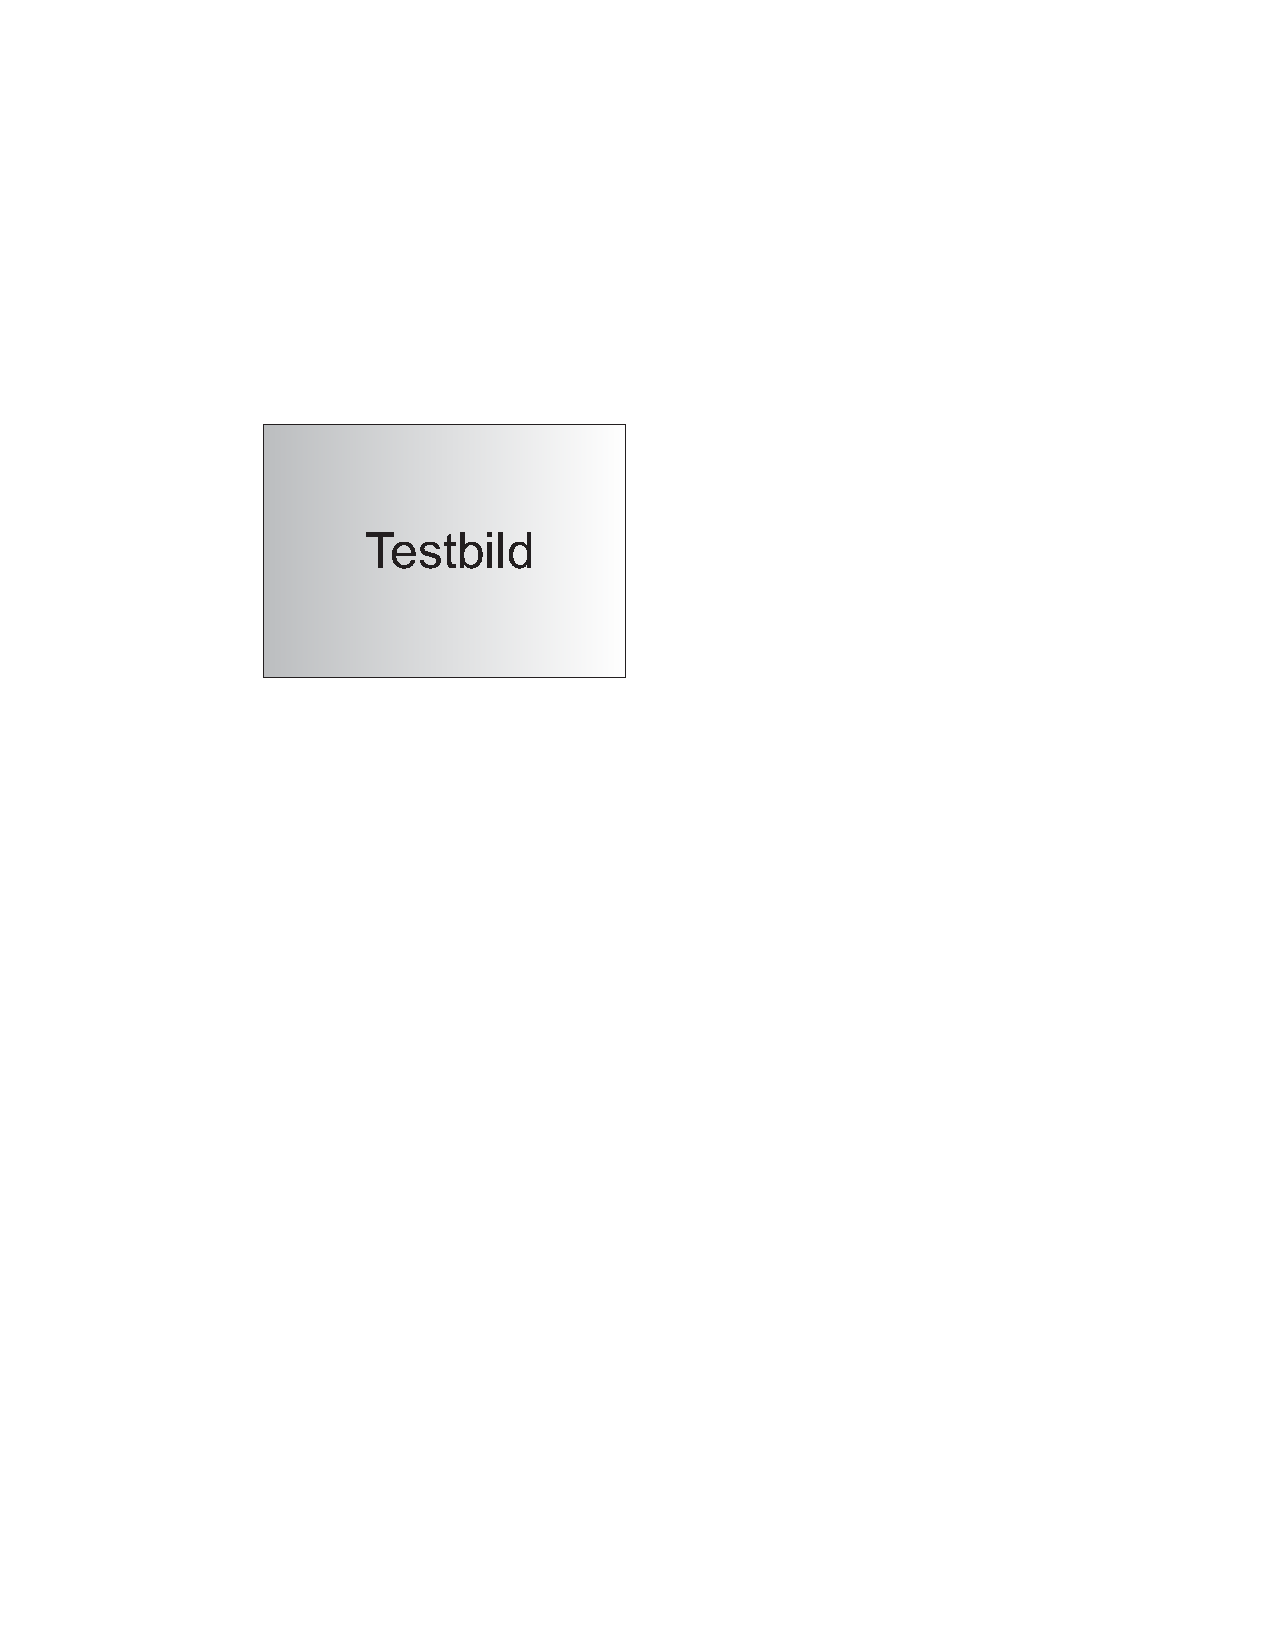
\includegraphics[scale=0.8]{bilder/testbild}\label{fig_testbild2_a}
    }
    \hspace{1.5cm}%
    \subfigure[testbild2b]
         {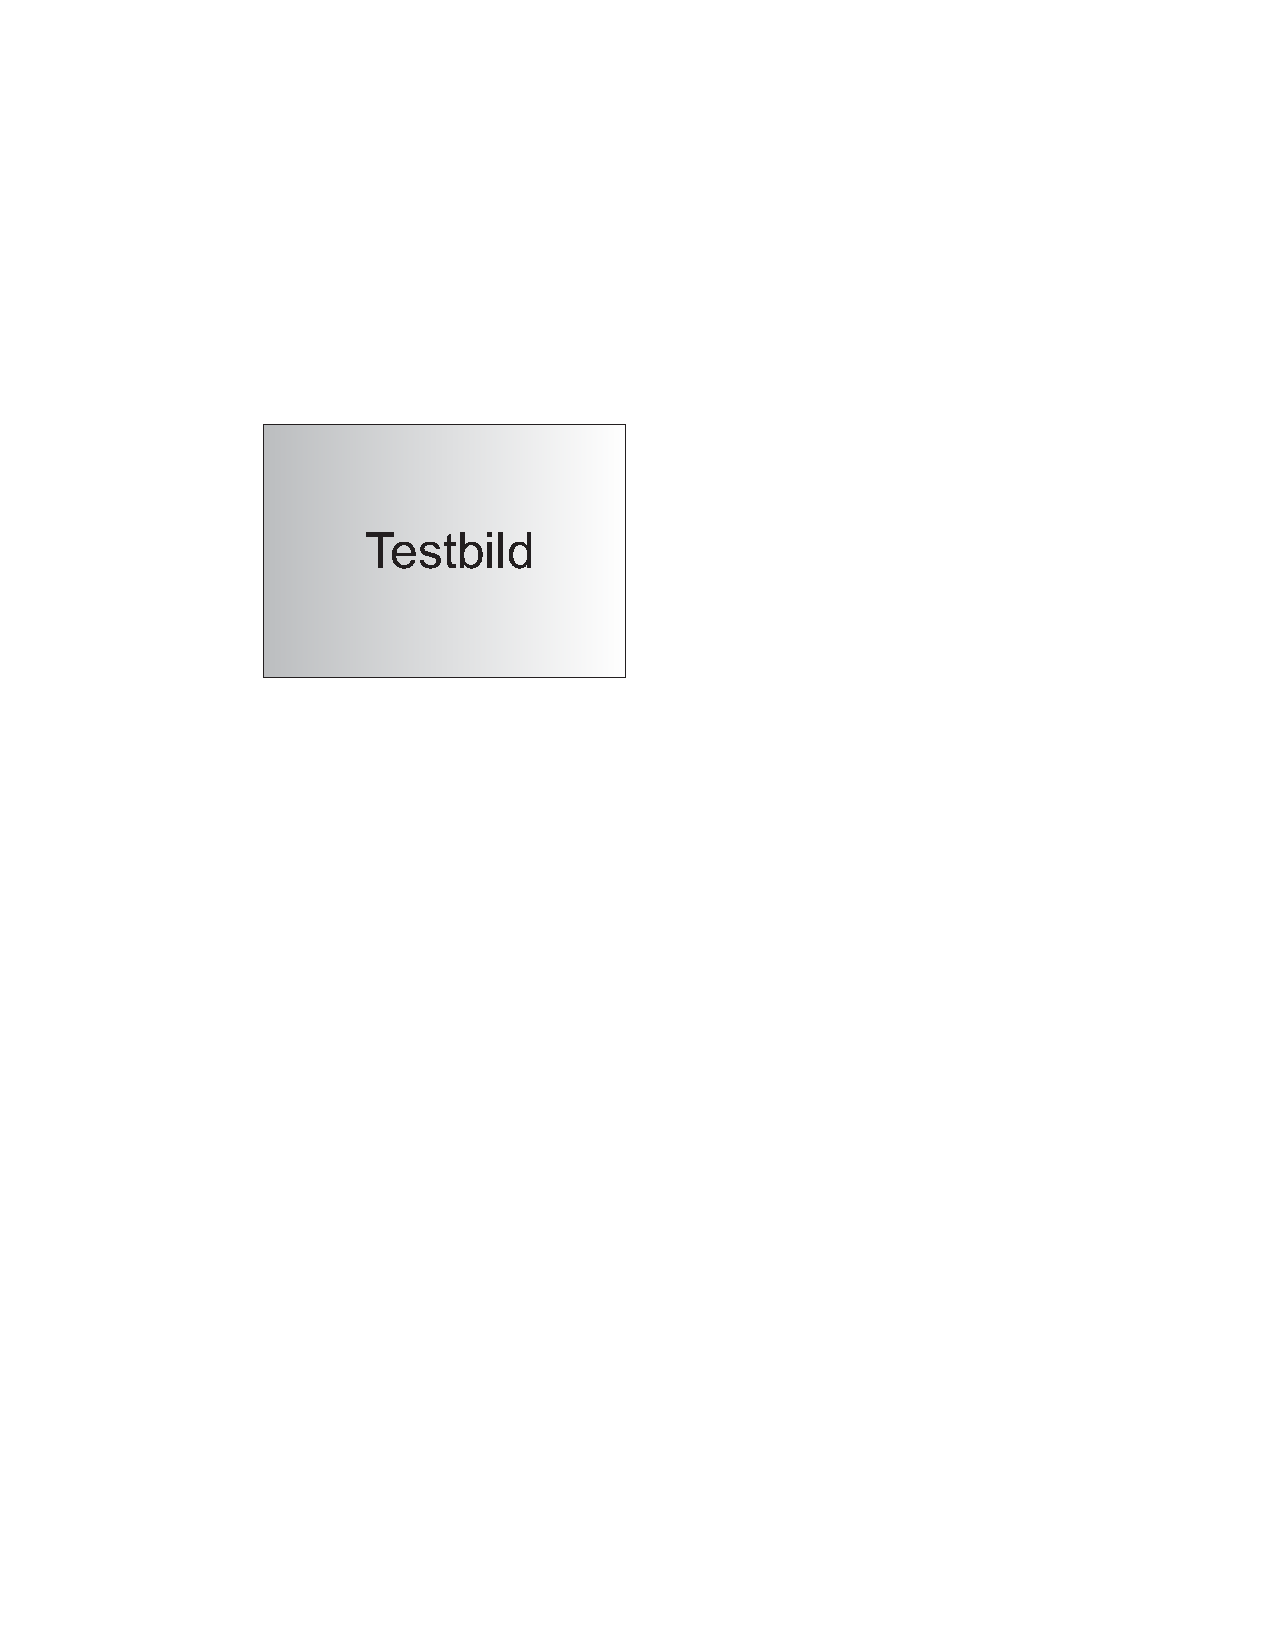
\includegraphics[scale=0.8]{bilder/testbild}\label{fig_testbild2_b}
    }\\
    \subfigure[testbild2c]
          {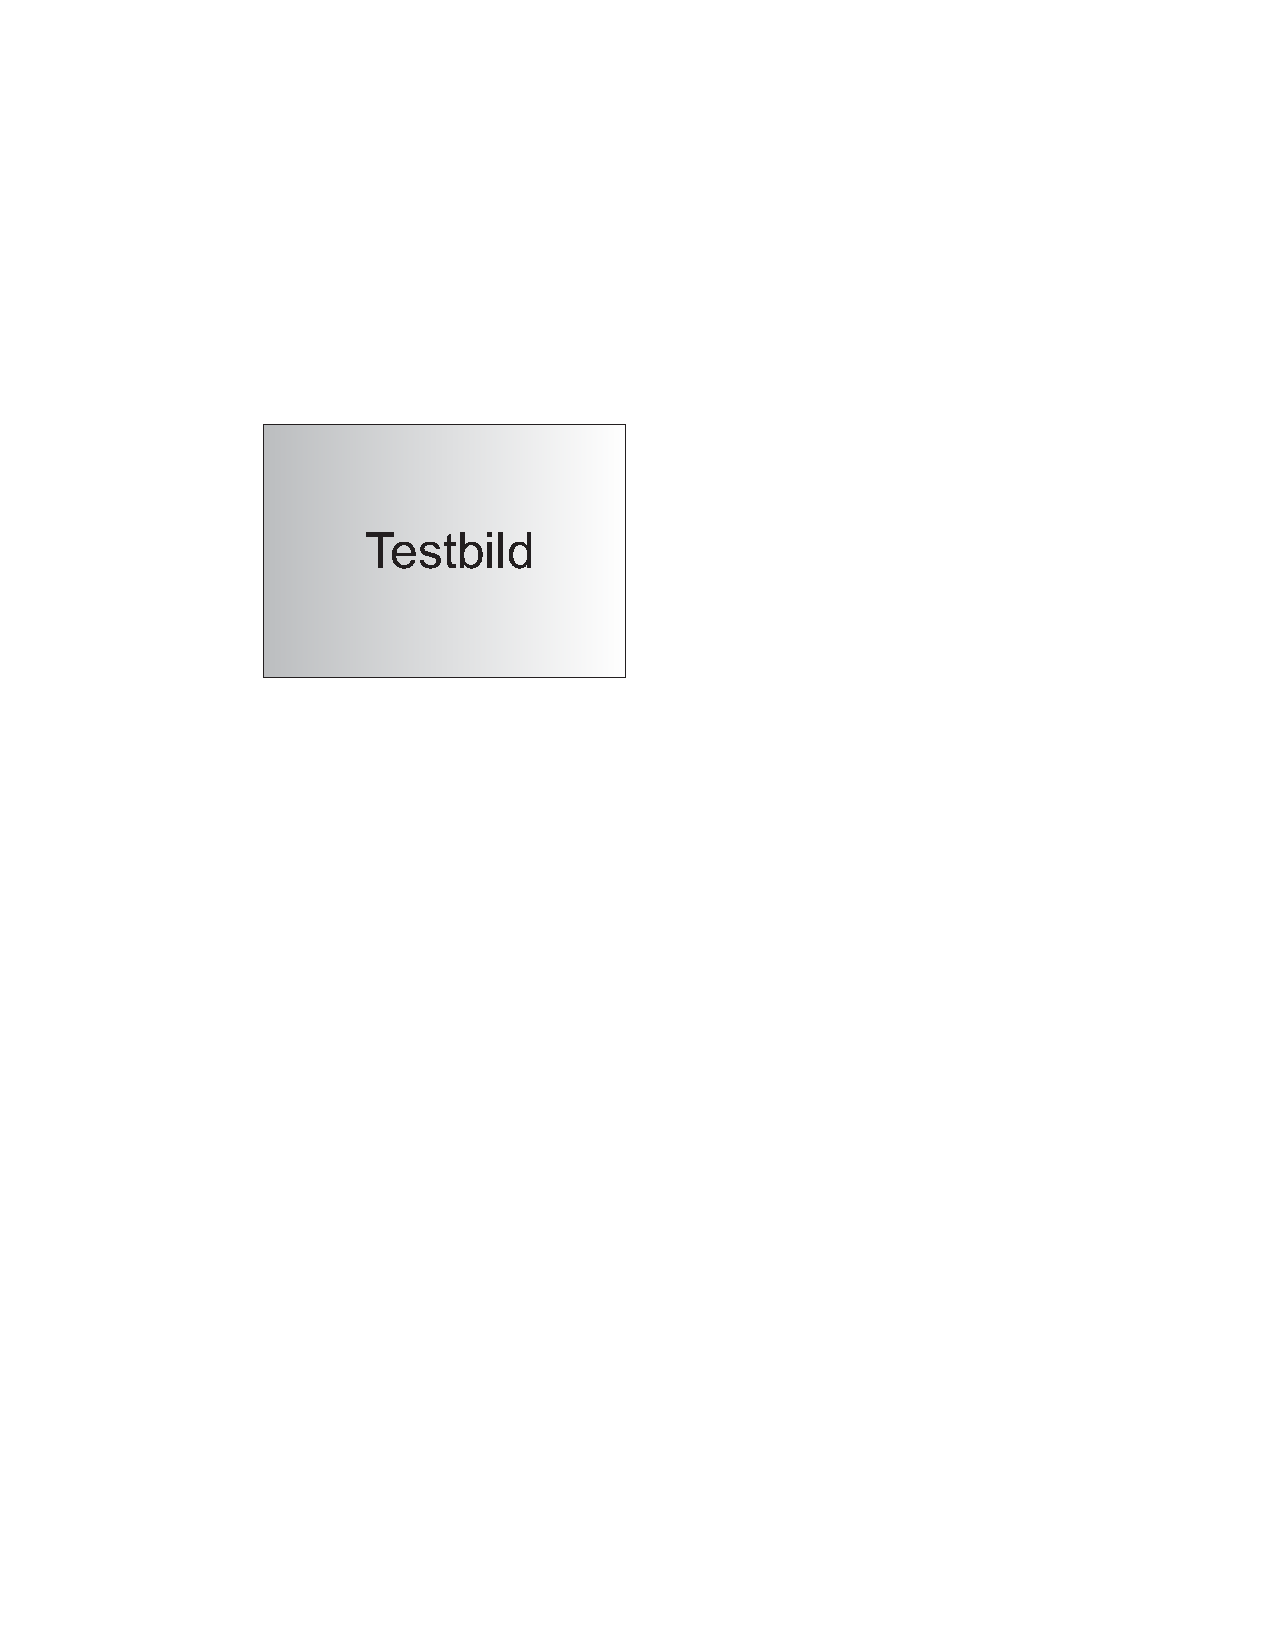
\includegraphics[scale=0.8]{bilder/testbild}\label{fig_testbild2_c}
    }
    \hspace{1.5cm}%
    \subfigure[testbild2d]
         {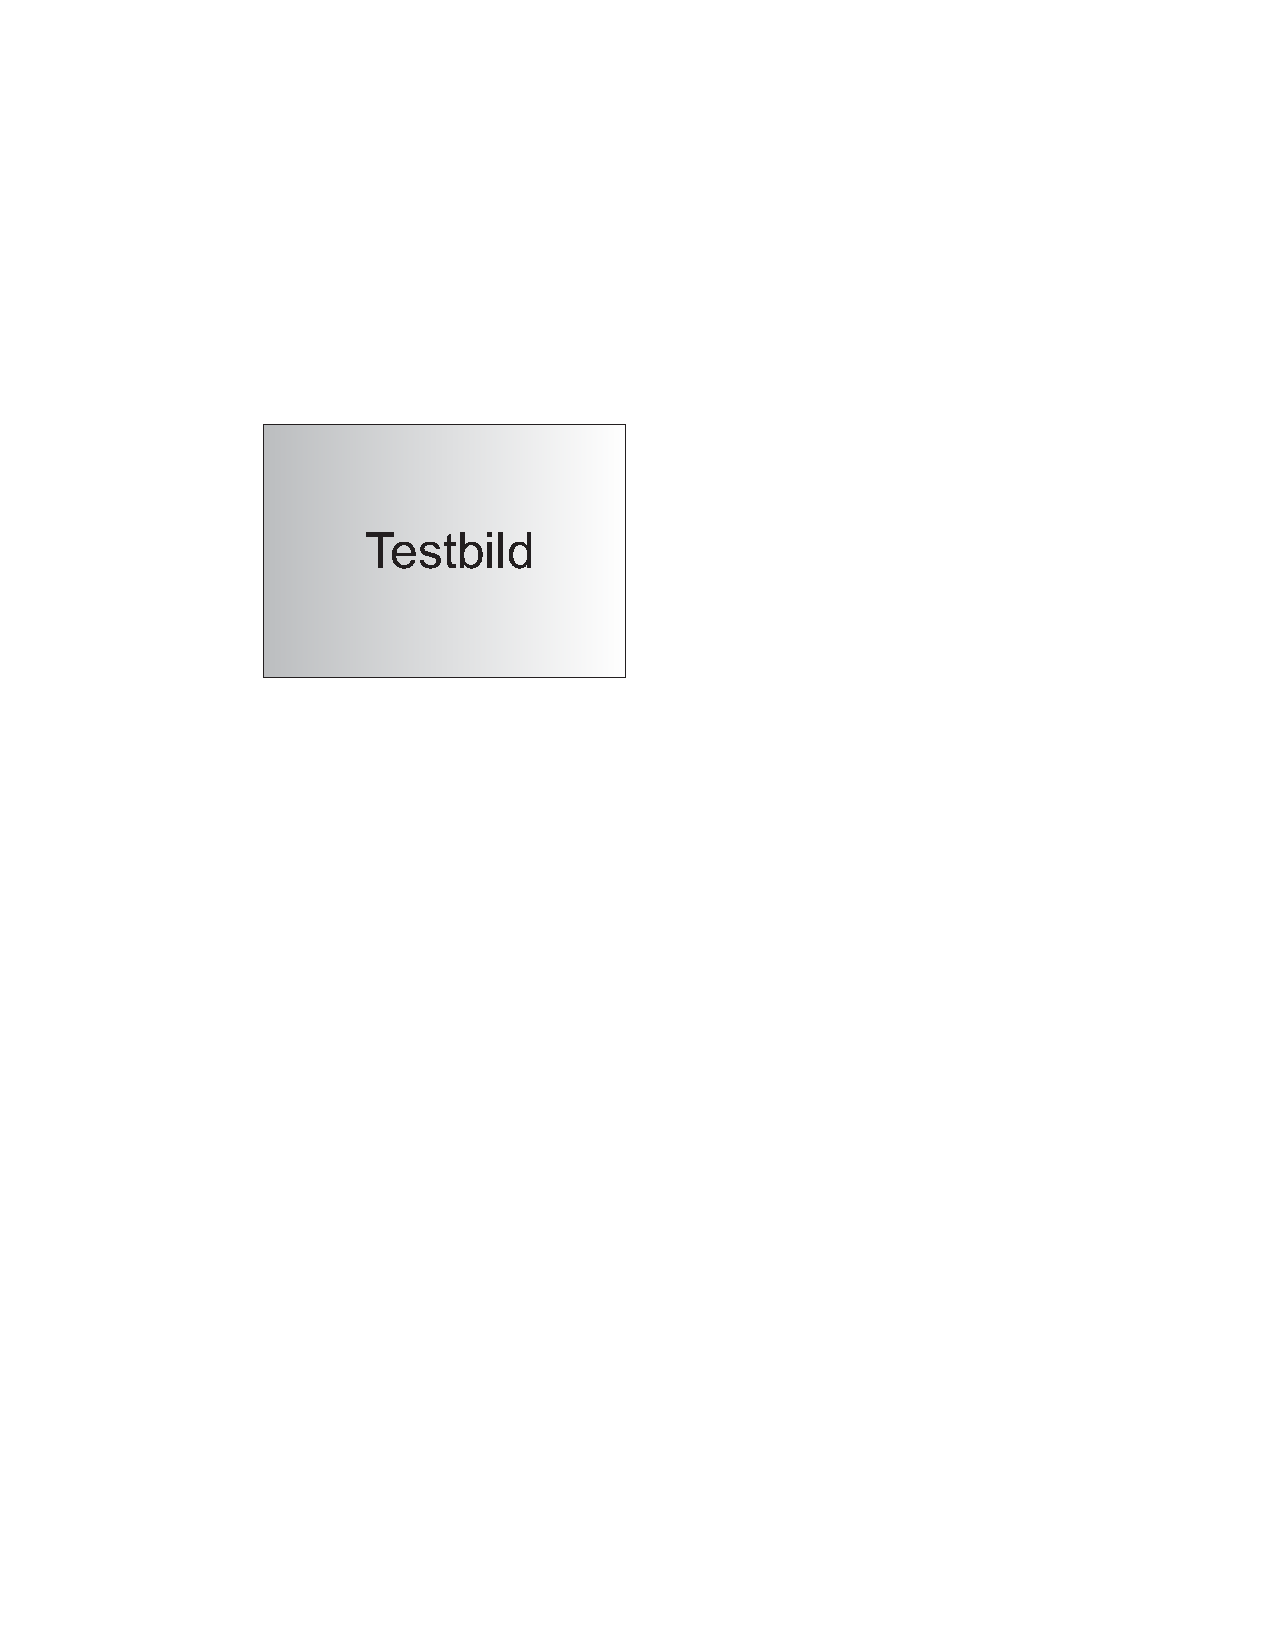
\includegraphics[scale=0.8]{bilder/testbild}\label{fig_testbild2_d}
    }\\
    \caption[Weitere Testbilder]{Weitere Testbilder}
        \label{fig_testbild2}
    \end{figure}

Er presste sich ganz eng an die Wand hinter ihm und hoffte, der
Verfolger würde ihn übersehen, als plötzlich neben ihm mit kaum
wahrnehmbarem Quietschen eine Tür im nächtlichen Wind hin und her
schwang. Könnte dieses der flehentlich herbeigesehnte Ausweg aus
seinem Dilemma sein? Langsam bewegte er sich auf die offene Tür
zu, immer dicht an die Mauer gepresst. Würde diese Tür seine
Rettung werden? Er hörte leise Schritte hinter sich. Das bedeutete
nichts Gutes. Wer würde ihm schon folgen, spät in der Nacht und
dazu noch in dieser engen Gasse mitten im übel beleumundeten
Hafenviertel? Gerade jetzt, wo er das Ding seines Lebens gedreht
hatte und mit der Beute verschwinden wollte! Hatte einer seiner
zahllosen Kollegen dieselbe Idee gehabt, ihn beobachtet und
abgewartet, um ihn nun um die Früchte seiner Arbeit zu
erleichtern? Oder gehörten die Schritte hinter ihm zu einem der
unzähligen Gesetzeshüter dieser Stadt, und die stählerne Acht um
seine Handgelenke würde gleich zuschnappen? Er konnte die
Aufforderung stehen zu bleiben schon hören. Gehetzt sah er sich
um. Plötzlich erblickte er den schmalen Durchgang. Blitzartig
drehte er sich nach rechts und verschwand zwischen den beiden
Gebäuden.

Er hörte \enquote{leise Schritte} hinter sich. Das bedeutete
nichts Gutes. Wer würde ihm schon folgen, spät in der Nacht und
dazu noch in dieser engen Gasse mitten im übel beleumundeten
Hafenviertel? Gerade jetzt, wo er das Ding seines Lebens gedreht
hatte und mit der Beute verschwinden wollte! Hatte einer seiner
zahllosen Kollegen dieselbe Idee gehabt, ihn beobachtet und
abgewartet, um ihn nun um die Früchte seiner Arbeit zu
erleichtern? Oder gehörten die Schritte hinter ihm zu einem der
unzähligen Gesetzeshüter dieser Stadt, und die stählerne Acht um
seine Handgelenke würde gleich zuschnappen? Er konnte die
Aufforderung stehen zu bleiben
schon hören.

Er hörte leise Schritte hinter sich. Das bedeutete nichts Gutes.Wer würde ihm schon folgen,
spät in der Nacht und dazu noch in dieser engen Gasse mitten im übel beleumundeten
Hafenviertel? Gerade jetzt, wo er das Ding seines Lebens gedreht hatte und mit der Beute
verschwinden wollte! Hatte einer seiner zahllosen Kollegen dieselbe Idee gehabt, ihn
beobachtet und abgewartet, um ihn nun um die Früchte seiner Arbeit zu erleichtern?
Oder gehörten die Schritte hinter ihm zu einem der unzähligen Gesetzeshüter dieser
Stadt, und die stählerne Acht um seine Handgelenke würde gleich zuschnappen? Er
konnte die Aufforderung stehen zu bleiben schon hören. Gehetzt sah er sich um. Plötzlich
erblickte er den schmalen Durchgang. Blitzartig drehte er sich nach rechts und verschwand
zwischen den beiden Gebäuden. Beinahe wäre er dabei über den umgestürzten Mülleimer
gefallen, der mitten im Weg lag. Er versuchte, sich in der Dunkelheit seinen Weg zu
ertasten und erstarrte: Anscheinend gab es keinen anderen Ausweg aus diesem kleinen
Hof als den Durchgang, durch den er gekommen war. Die Schritte wurden lauter und
lauter, er sah eine dunkle Gestalt um die Ecke biegen. Fieberhaft irrten seine Augen durch
die nächtliche Dunkelheit und suchten einen Ausweg. War jetzt wirklich alles vorbei,
waren alle Mühe und alle Vorbereitungen umsonst? Er presste sich ganz eng an die Wand
hinter ihm und hoffte, der Verfolger würde ihn übersehen, als plötzlich neben ihm mit
kaum wahrnehmbarem Quietschen eine Tür im nächtlichen Wind hin und her schwang.
Könnte dieses der flehentlich herbeigesehnte Ausweg aus seinem Dilemma sein? Langsam
bewegte er sich auf die offene Tür zu, immer dicht an die Mauer gepresst. Würde diese
Tür seine Rettung werden?

%


%% erklaerung.tex
\pagestyle{empty}

\normalsize


\begin{center}
{\bf Eidesstattliche Versicherung }
\end{center}
~\\
\noindent \rule{10cm}{0.4pt}   \hspace{1.5cm} \noindent \rule{3.5cm}{0.4pt}  \\
      {Name, Vorname}    \hspace{8.7cm} {Matrikelnummer}  

\vspace{0.5cm}
Ich versichere hiermit an Eides statt, dass ich die vorliegende Bachelorarbeit/Masterarbeit* mit
dem Titel

\vspace{0.5cm}
\noindent \rule{15cm}{0.4pt}

\vspace{0.5cm}

\noindent \rule{15cm}{0.4pt}

\vspace{0.5cm}
\noindent \rule{15cm}{0.4pt}
~\\
selbstst\"andig und ohne unzul\"assige fremde Hilfe erbracht habe. Ich habe
keine anderen als die angegebenen Quellen und Hilfsmittel benutzt sowie
w\"ortliche und sinngem\"aße Zitate kenntlich gemacht. Die Arbeit hat in
gleicher oder \"ahnlicher Form noch keiner Pr\"ufungsbeh\"orde vorgelegen.
~\\

\noindent \rule{5cm}{0.4pt}   \hspace{3.5cm} \noindent \rule{6cm}{0.4pt}  \\
      {Ort, Datum}    \hspace{6.5cm} {Unterschrift}  \vspace{0.2cm}

      ~ \hspace{8.5cm} {* Nichtzutreffendes bitte streichen}

\vspace{0.5cm}
{\bf Belehrung:}

Wer vors\"atzlich gegen eine die T\"auschung \"uber Pr\"ufungsleistungen
betreffende Regelung einer Hochschulpr\"ufungsordnung verst\"oßt, handelt
ordnungswidrig. Die Ordnungswidrigkeit kann mit einer Geldbuße von bis zu
50.000,00 € geahndet werden. Zust\"andige Verwaltungsbeh\"orde für die
Verfolgung und Ahndung von Ordnungswidrigkeiten ist der Kanzler/die Kanzlerin
der Technischen Universit\"at Dortmund. Im Falle eines mehrfachen oder
sonstigen schwerwiegenden T\"uschungsversuches kann der Prüfling zudem
exmatrikuliert werden. (§ 63 Abs. 5 Hochschulgesetz - HG - )

Die Abgabe einer falschen Versicherung an Eides statt wird mit Freiheitsstrafe bis zu 3 Jahren
oder mit Geldstrafe bestraft.

Die Technische Universit\"at Dortmund wird gfls. elektronische
Vergleichswerkzeuge (wie z.B. die Software „turnitin“) zur \"Uberpr\"ufung von
Ordnungswidrigkeiten in Pr\"ufungsverfahren nutzen.

Die oben stehende Belehrung habe ich zur Kenntnis genommen:
~\\

\noindent \rule{5cm}{0.4pt}   \hspace{3.5cm} \noindent \rule{6cm}{0.4pt}  \\
      {Ort, Datum}    \hspace{6.5cm} {Unterschrift}  \vspace{0.2cm}

% Anhang ---------------------------------------------------------------
%
\cleardoublepage
\appendix


%========================================================================================
% TU Dortmund, Informatik Lehrstuhl VII
%========================================================================================

\chapter*{Appendix}




% Abbildungsverzeichnis -------------------------------------------------
%
\listoffigures
\addcontentsline{toc}{chapter}{List of Figures }
\cleardoublepage

% Algorithmenverzeichnis ------------------------------------------------
%
\listofalgorithms
\addcontentsline{toc}{chapter}{List of Algorithms}
\cleardoublepage

% Quellcodeverzeichnis --------------------------------------------------
%
\renewcommand{\lstlistlistingname}{List of Source Codes}
\lstlistoflistings
\addcontentsline{toc}{chapter}{List of Source Codes}
\cleardoublepage

% Literaturverzeichnis
%
\bibliographystyle{abbrv}
\bibliography{literatur}
\addcontentsline{toc}{chapter}{\bibname}

% ----------------------------------------------------------------------


%\cleardoublepage
%\addcontentsline{toc}{chapter}{Eidesstattliche Versicherung}
%\include{Eidesstattliche_Versicherung.pdf}
\clearpage
\pagestyle{empty}
\addcontentsline{toc}{chapter}{Eidesstattliche Versicherung}
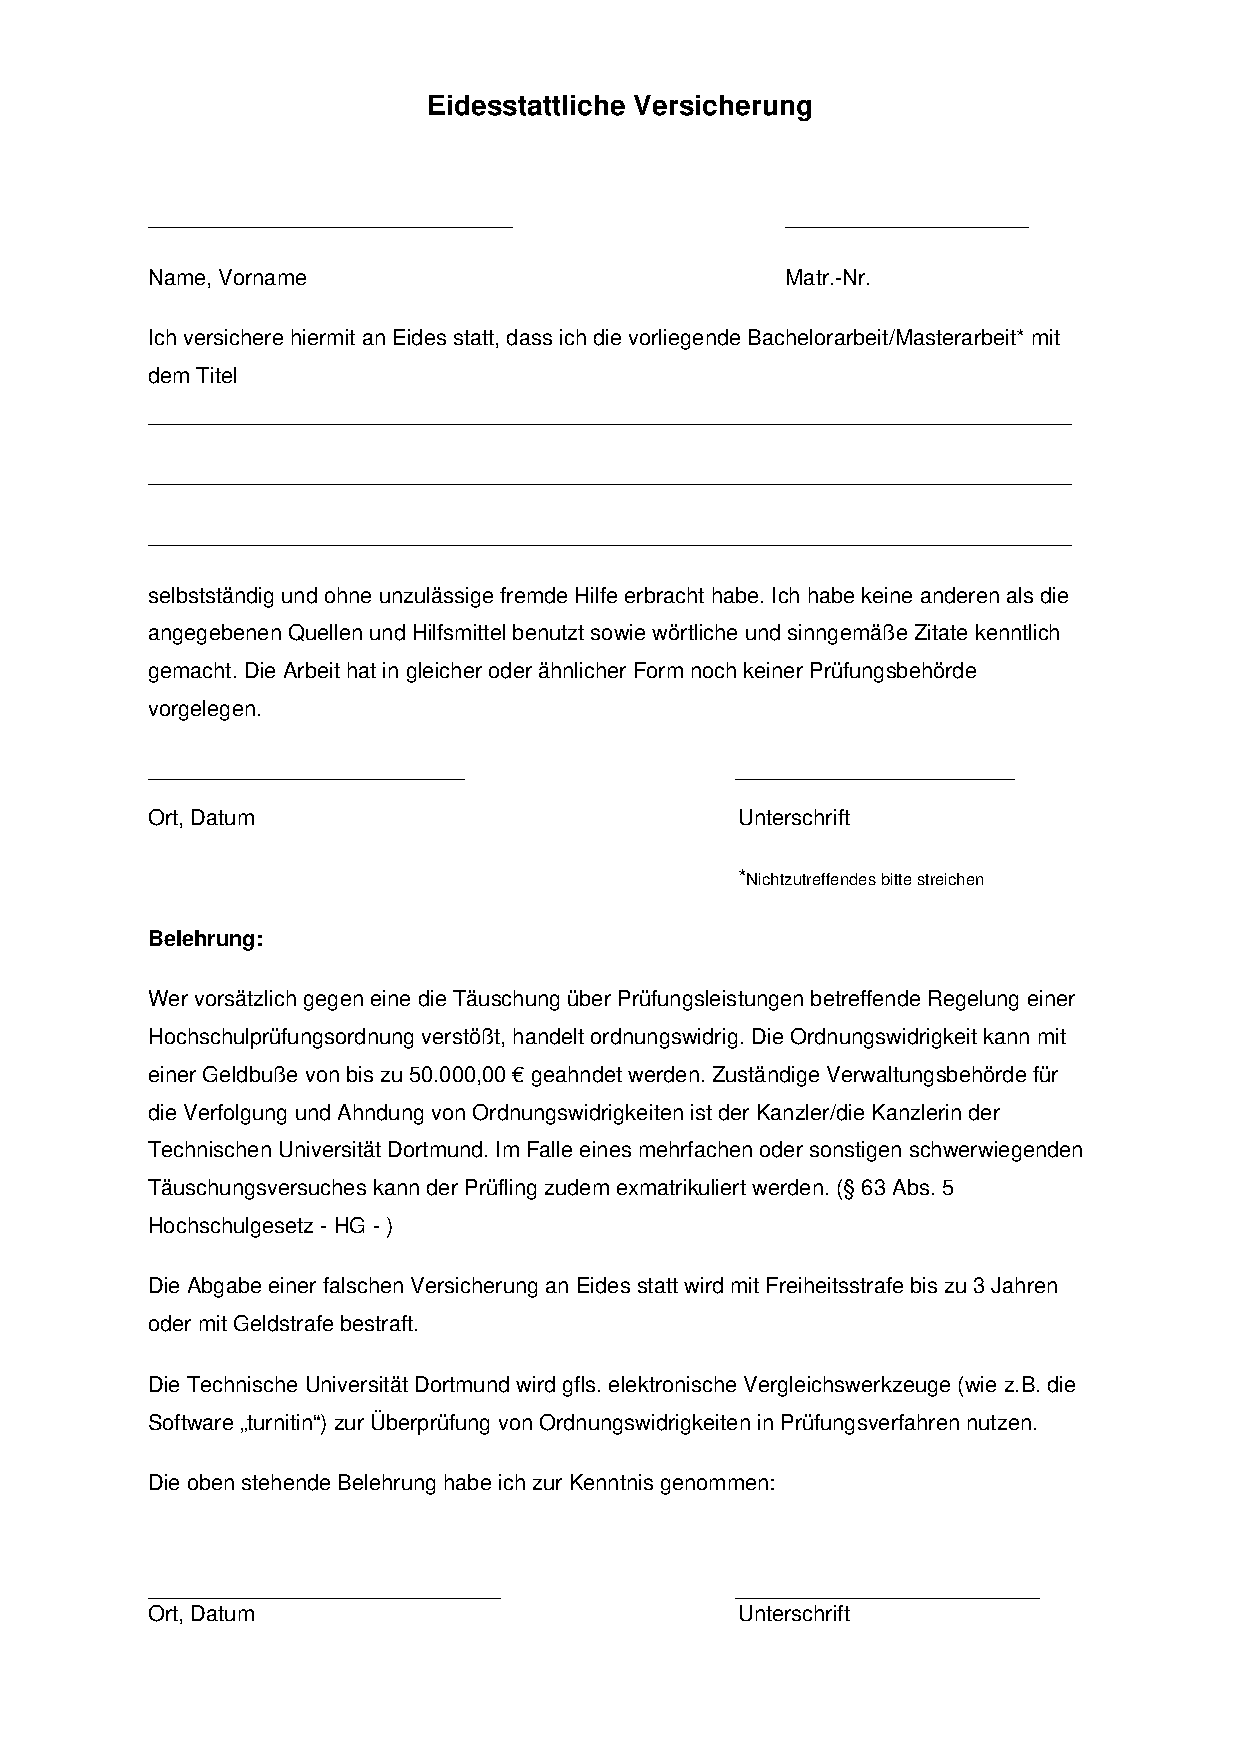
\includegraphics[trim = 20mm 20mm 20mm 10mm, clip,
width=\textwidth]{Eidesstattliche_Versicherung.pdf}


%%========================================================================================
% TU Dortmund, Informatik Lehrstuhl VII
%========================================================================================

\chapter*{Appendix}




\end{document}
